% !TEX encoding = UTF-8 Unicode
\section{Cancer metabolism}

Compared with normal, differentiated, quiescent cells, proliferative tumor cells exhibit distinct metabolic profile, involving the generation of energy from aerobic glycolysis, a phenomenon called "Warburg Effect" initially described by Otto Warburg at last century \cite{warburg_respiratory_1956,warburg_origin_1956,warburg_metabolism_1931}. In proliferative tissues or tumors, quickly dividing cells ferment a major fraction of glucose into secreted lactate and inefficiently produce ATP from glycolysis (2 ATP molecules per glucose) instead of the mitochondrial oxidative phosphorylation in mitochondria (\textasciitilde36 ATP molecules per glucose). 

The preference over fermentation in glucose utilization was first discovered in yeast \cite{ward_metabolic_2012}. Otto Warburg's findings in proliferative ascites tumor cells established the glucose utilization into lactate secretion, even under hyperoxia condition. Warburg and his contemporaries postulated that the aerobic glycolysis is the specific marker for cancer cells, and defective mitochondria are responsible for the energy production switch to glycolysis. The "Warburg Effect" is generally true for the majority of cancer cells, and extensively applied in the clinical diagnosis for tumor detection in human by the \textsuperscript{18}F-deoxyglucose positron emission tomography (FDG-PET)  \cite{ward_metabolic_2012}.

Besides extensive clinical applications of the Warburg effect, recent studies in cancer cells showed that most of the cancer cells are not defective in mitochondrial function, including the oxidative phosphorylation for efficient ATP generation  \cite{fantin_attenuation_2006,moreno-sanchez_energy_2007,weinhouse_warburg_1976}. These observations suggest the existence of an alternative explanation for the ATP production switch from oxidative phosphorylation to aerobic glycolysis, which is the altered metabolism in cancer cells for supporting anabolic growth requirements in the proliferation, including fast ATP generation, massive biosynthesis of macromolecules and tight maintenance of the cellular redox status  \cite{cairns_regulation_2011}. It is now clear that the metabolism change in the cancer cells is driven by the growth factor signaling transduction, and not the secondary indirect consequences upon the increasing demand from fast growth and dividing, but rather tightly regulated metabolism reprogramming to increase the nutrient uptake and flux under the control of activated oncogenes or inactivated tumor suppressors  \cite{ward_metabolic_2012}. This new understanding of cancer metabolism has become one of the hallmarks of cancer  \cite{hanahan_hallmarks_2011}.

\subsection{Metabolism switch in quiescent vs proliferative cell}

Most of the non-proliferative cells in differentiated tissues are quiescent and producing ATP efficiently via the oxidative phosphorylation in mitochondria. In the presence of oxygen, these cells preferentially generate ATP from oxidation of glucose into CO\textsubscript{2} by oxidizing glycolytic product pyruvate in the TCA cycle happening in mitochondria. Besides a net gain of 2 ATP generated from the glycolysis, NADH, GTP and FADH\textsubscript{2} are produced during sequential oxidation of the pyruvate in the TCA cycle. These products from the TCA cycle are fueling the oxidative phosphorylation complexes I-V to generate \textasciitilde36 ATP/glucose in total. Under anaerobic conditions, differentiated cells could produce a large amount of lactate from glycolysis while the oxidative phosphorylation is bypassed.

In contrast, cancer cells utilize 10\% glucose for the biosynthetic pathway upstream of pyruvate production and the rest 90\% glucose for pyruvate production \cite{ward_metabolic_2012,heiden_understanding_2009}. Among this 90\% glucose, 5\% of them will be metabolized via oxidative phosphorylation and the rest 85\% of them will be converted to lactate. This process could only generate \textasciitilde4 ATP/glucose (Figure~\ref{fig:fig1.4}). One of the possible reasons for employing this low-efficiency ATP production by cancer cells is that the nutrient availability is not an issue for them. Cancer cells live in an environment having continuous supply of glucose and other nutrients. There are evidences that the ATP production is never a limiting factor during the cell division \cite{deberardinis_biology_2008,christofk_m2_2008}. Even highly stimulated to growth and dividing, cancer cells are still able to maintain high ATP/ADP and NADH/NAD\textsuperscript{+} ratios.

\begin{figure}[htbp]
\centering
\includegraphics[width=0.5\textwidth]{figs/fig1-4 aerobic glycolysis.pdf}
\caption[Glucose metabolism in cancer cells]{\footnotesize Glucose metabolism in cancer cells. Modified based on Vander Heiden et al. \cite{heiden_understanding_2009}.}
\label{fig:fig1.4}
\end{figure}

Beyond the ATP requirement, cancer cells also need double their cellular contents for the cell division. There are huge needs for nucleotides, amino acids, and lipids for the macromolecular biosynthesis and new membrane formation. Although ATP is indispensable for most of the biomass accumulation reactions, other intermediate metabolites are also needed. For example, the palmitate synthesis for reconstituting new cellular membrane, requires 8 molecules of acetyl-CoA as the carbon source, 14 molecules of NADPH for the reducing power, as well as 7 molecules of ATP. One molecule of glucose could generate up to 36 ATP, or 30 ATP plus 2 NADPH through phosphate pentose pathway, or just provide 6 carbons for macromolecular biosynthesis. Now back to the palmitate synthesis, one molecule of glucose could provide \textasciitilde5 times ATP needed for 16-carbon fatty acid synthesis, or 1/7 of the NADPH needed for it. There is a 35-fold asymmetry between the need for ATP and that for NADPH, given that 3 additional glucose for making the acetyl-CoA as the carbon source for the palmitate synthesis \cite{nelson_lehninger_2013}. Thus, during the cell proliferation, a majority of glucose can not undergo the oxidative phosphorylation to generate ATP, otherwise the resulting high ratio of ATP/ADP will negatively control the flux of glycolysis and compromise the production of acetyl-CoA and NADPH, which leads to the impaired biomass accumulation. The "by-product" lactate could also be converted into glucose again in the liver by the Cori cycle \cite{nelson_lehninger_2013}.


\subsection{Signaling in metabolism reprogramming}

Recently, there were increasing evidences support the hypothesis that the metabolic reprogramming is a hallmark of the tumor development and the primary consequence of the mutation in oncogenes and tumor suppressor genes \cite{hanahan_hallmarks_2011,ward_metabolic_2012}. The cancer cell proliferation not only relies on a large amount of energy consumption, but also needs other build blocks for the cell growth, such as amino acids for the protein synthesis and fatty acids for the lipid bilayer formation. For these purposes, the cell metabolism must undergo a massive reprogramming to fulfill the increased anabolic demand for the cell growth and division. Interestingly, the cancer cell metabolic reprogramming and metabolic syndromes such as type 2 diabetes and hepatosteatosis (fatty liver), are sharing a broad range of signaling pathways in etiology. One of these is the Insulin/PI3K/AKT/mTOR pathway. Activation of PI3K/AKT is probably the most prominent lesion in various types of cancer. mTOR, a downstream target of PI3K/AKT, is well-characterized for its role in enhancing the protein synthesis, glycolysis and lipogenesis via the S6K, HIF1\textalpha{} and SREBP-1 respectively \cite{duvel_activation_2010,hagiwara_hepatic_2012,sun_mammalian_2011}. Dissecting the signaling network behind the insulin signaling could potentially reveal more pharmaceutical targets for treating both cancers and metabolic syndromes. 



\section{Liver metabolism}

The liver is the largest organ in the body, contributing about 2\% total body weight in human and 5\% in mouse \cite{hall_guyton_2010}. The liver is a lobular structure composed of many cylindrical \textit{liver lobules} as the basic function unit. Each unit containing 3 types of cell: hepatocytes, endothelial cells and Kupffer cells (local macrophage cells in the liver). The liver performs many important functions in physiology including:
\begin{inparaenum}[(1)]
\item the filtration and storage of blood
\item the metabolism of carbohydrates, lipids, proteins, hormones and foreign chemicals
\item the bile acid synthesis
\item the vitamin and iron storage
\item the synthesis of serum proteins, such as the albumin, coagulation factors
\end{inparaenum} \cite{hall_guyton_2010}.

In this thesis project, the liver glucose and lipid metabolism are the main focuses. The liver is especially essential organ for maintaining the blood glucose level. The liver can serve as a glucose buffer. In the postprandial phase, a large amount of blood glucose is transported into the liver for the glycogen synthesis and lipid \textit{de novo} synthesis \cite{moore_regulation_2012}, which allow the removal of excess blood glucose and returning into the blood when the glucose level drops below the normal. The liver can also synthesize glucose via gluconeogenesis when blood glucose falls below the normal. During this process, a large amount of amino acids and glycerol released from triglycerides are converted into glucose and released into circulation to maintain the normal level of blood glucose. 

For lipid metabolism, the liver is the major organ for a certain aspect of the fat metabolism, including:
\begin{inparaenum}[(1)]
\item the fat oxidation
\item the synthesis of lipoproteins, cholesterol and phospholipids
\item the free fatty acid and triglyceride synthesis from carbohydrates and proteins
\end{inparaenum} \cite{hall_guyton_2010}. The major sites for \textit{de novo} lipogenesis are the liver and adipose tissues. In the liver, the products from lipogenesis are either stored as lipid droplets in the liver or secreted in the form of \gls{vldl} (\textbf{V}ery \textbf{L}ow \textbf{D}ensity \textbf{L}ipoprotein), which delivers the endogenous derived lipids to peripheral organs.   

\subsection{Liver glucose regulation}

After digestion in the alimentary tract, final products of carbohydrates are glucose, galactose and fructose. Much of the fructose and all of the galactose are interconverted into glucose in the liver. Thus, the glucose becomes the dominant carbohydrate circulating in the blood. 

In the postprandial phase, the liver plays a critical role in nutrient absorption and metabolism, since it is the first barrier to filter all ingested nutrients through the hepatic port vein. This process filters out micro-organisms absorbed together with nutrients, such as bacteria, fungi, viruses and parasites. As the first access to nutrients, the liver is exposed to higher nutrient levels than peripheral organs. A large amount of glycogen is synthesized in the liver in order to relieve the modest hyperglycemia after meal for a normal individual. In addition, the liver also produces glucose to maintain the glucose homeostasis during the fasting state. In a diabetic person, the liver is one of the major culprits for hyperglycemia due to the impaired balance between glucose uptake and production in the liver \cite{krssak_alterations_2004}. 

\subsubsection{Liver glucose uptake}

In the postprandial phase or during the high glucose load via oral or enteral delivery, the liver shifts the balance toward more glucose uptake than endogenous glucose production (\gls{nhgu} (\textbf{N}et \textbf{H}epatic \textbf{G}lucose \textbf{U}ptake) shifts from modest to high in dog \cite{abumrad_absorption_1982,moore_sources_1991}.). Glucose uptake experiments in human and dog have shown that the liver \gls{nhgu} takes up 25--40\% of the administered glucose, while muscle and adipose tissues take one-third, and the non-insulin-sensitive glucose obligating tissues (brain, red blood cells, etc.) absorb the remaining one third (Figure~\ref{fig:fig1.2}). Actually, the liver NHGU underestimates the role of the liver in glycemic control. The total capacity of the liver in glucose disposal upon oral glucose load is about 60--65\%, demonstrates the great importance of the liver in the glucose clearance and production \cite{moore_regulation_2012}. Once taken up by the liver, glucose is converted to glucose-6-phosphate by the liver glucokinase (L-GCK). Unlike other hexokinases, the L-GCK is not inhibited by glucose-6-phosphate. This allows the active glycogen storage in the postprandial phase.

\begin{figure}[htbp]
\centering
\includegraphics[width=1\textwidth]{figs/fig1-2 liver glucose.png}
\caption[Glucose redistribution in whole body]{\footnotesize Glucose absorption among metabolism related tissues. Modified based on Moore et al. \cite{moore_regulation_2012}.}
\label{fig:fig1.2}
\end{figure}


\subsubsection{Glycolysis for energy and metabolite intermediate production}

Glucose-6-phosphate is further metabolized in glycolysis or stored in the form of glycogen. Glycolysis converts glucose into pyruvate with 2 ATP and 2 NADH released from one glucose molecule. The pyruvate is further decarboxylated to acetyl-CoA and then submitted for the TCA cycle or \textit{de novo} lipogenesis. The pentose phosphate pathway (PPP) is another way of metabolizing glucose, which generates NADPH as the antioxidant or reducing equivalent for the \textit{de novo} lipogenesis and cholesterol synthesis.

\subsubsection{Glycogen storage and breakdown in the liver}

After the glucose is absorbed into the liver, it can be metabolized in glycolytic pathway to release energy and building blocks for the protein and lipid synthesis, or it can be stored as glycogen for future use such as releasing glucose in fasting state. The liver can store as much as 5--8\% of its weight as glycogen. The conversion of glucose to glycogen allows the liver cell store large amount of carbohydrates without increasing the intracellular osmotic pressure.

%\paragraph{Glycogenesis for glycogen formation}
The chemical process of glycogen synthesis is that glucose-6-phosphate is interconverted into glucose-1-phosphate; this is converted to uridine diphosphate glucose, which is finally synthesized into glycogen by glycogen synthase (GS).
%There are several enzymes involved in this process:
%\begin{inparaenum}[(1)]
%\item the phosphoglucomutase for reversible interconversion between glucose-6-phosphate and glucose-1-phosphate;
%\item the UTP-glucose-1-phosphate uridylyltransferase for UDP-glucose synthesis from UTP and glucose-1-phosphate;
%\item the glycogenin for initiating glycogen synthesis by catalyzing the attachment of a glucose molecule to one of its own tyrosine residues;
%\item the glycogen synthase (GS) for catalyzing the elongation of glycogen chains;
%\end{inparaenum}.
The GS can be regulated by several pathways. The glucose-6-phosphate can allosterically activate GS. The phosphorylation of GS can also reduce its activity. Numerous kinases have been shown to regulate GS via phosphorylation \cite{palm_regulation_2013}. The phosphorylation of GS occurs both in the primary and secondary phosphorylation sites. Primary phosphorylation events are initiated by the phosphorylase kinase, \gls{pka}, \gls{AMPK}, \gls{pkc}, \gls{camk2}, and \gls{ck2}. Secondary phosphorylation events are initiated by the \gls{gsk3} and \gls{ck1}. 

%\paragraph{Glycogenolysis for glycogen removal}

In fasting state, the liver produces glucose for the whole body by breaking down glycogen into glucose in a process called glycogenolysis. This process is catalyzed by the glycogen phosphorylase. The glycogen phosphorylase is regulated by the allosteric activation of AMP and activated by the phosphorylation via PKA. The product from glycogenolysis is glucose-1-phosphate, which will be further converted to glucose-6-phosphate by phosphoglucomutase. And the glucose 6-phosphatase remove the phosphate group from glucose-6-phosphate to produce glucose which will be transported out of the liver. 


\subsection{Liver lipid metabolism}

\subsubsection{Dietary lipid absorption}

During the digestion, triglycerides from the food are split into monoglycerides and fatty acids, which are re-esterified in the intestinal epithelial cell into triglycerides and released into the lymphatic system as lipoprotein droplets called chylomicrons (Figure~\ref{fig:fig1.3}). Chylomicrons also contain cholesterol and phospholipids absorbed from the food. The half-life of chylomicrons is less than 1 hour. Most of the chylomicrons are cleared out in the capillary of muscle, adipose and liver by the action of the lipoprotein lipase (LPL). The remnants of chylomicron are absorbed by the liver via the LDL (\textbf{L}ow \textbf{D}ensity \textbf{L}ipoprotein) receptor, LDL receptor-related protein (LRP) and scavenger receptor B-1 mediated endocytosis. The engulfed chylomicrons in hepatocytes are digested in the lysosome to release glycerol, fatty acids, cholesterol, which are recycled into VLDL.



\subsubsection{Lipoprotein particle for lipid transportation and redistribution}

Besides chylomicrons, there are four major types of lipoprotein particles circulating in the plasma (Figure~\ref{fig:fig1.3}). Most of these lipoprotein particles are synthesized by the liver and employed to redistribute triglycerides, cholesterols, and phospholipids among peripheral tissues. These lipoprotein particles are classified based on their density measured in the ultracentrifugation:
\begin{inparaenum}[(1)]
\item the \gls{vldl} is synthesized in the liver and containing the highest amount of triglycerides (\textasciitilde70\%) and modest amount of cholesterol (\textasciitilde7.5\%) and phospholipids \cite{ginsberg_regulation_2005};
\item the \gls{idl} (\textbf{I}ntermediate \textbf{D}ensity \textbf{L}ipoprotein) is derived from the VLDL, in which triglycerides are partially removed;
\item the \gls{ldl} is derived from the IDL, in which almost all triglycerides are absorbed by peripheral tissues, left with very high amount of cholesterol (\textasciitilde45\%) \cite{ginsberg_regulation_2005};
\item the \gls{hdl} (\textbf{H}igh \textbf{D}ensity \textbf{L}ipoprotein) is synthesized in the liver or intestine epithelium, containing high concentration of protein (\textasciitilde50\%) and modest amount of cholesterols (\textasciitilde20\%) and phospholipids \cite{ginsberg_regulation_2005};
\end{inparaenum}.

\begin{figure}[!tb]
\centering
\includegraphics[width=1\textwidth]{figs/fig1-3 liver lipid.png}
\caption[Lipid redistribution in the whole body]{\footnotesize The lipid absorption and lipoprotein particle redistribution among metabolism related tissues.}
\label{fig:fig1.3}
\end{figure}

In contrast to the chylomicron for exogenous lipid transportation, the primary function of the VLDL is transporting endogenous liver-derived triglycerides and cholesterols to peripheral tissues such as the muscle and adipose tissues. As partially digested lipoprotein from VLDL, the IDL is either taken up by the liver or continually circulating in the plasma to convert into LDL. The LDL contains high amount of cholesterol, which is also called the "bad cholesterol" in comparison to the "good cholesterol" in HDL. Increasing blood cholesterol from LDL is a strong risk factor for causing the atherosclerosis. The HDL is responsible for the delivery of the cholesterol to peripheral tissues and the removal of excess cholesterol from the plasma in a process called the reverse cholesterol transport \cite{mahley_putting_2006,van_der_velde_reverse_2010}.

\subsubsection{\textit{de novo} lipogenesis in the liver}

Whenever a greater amount of the carbohydrate than it can be used immediately such as in glycolysis or stored in the form of glycogen, the excess is quickly converted to triglycerides. Most of the triglyceride synthesis occurs in the liver, while a small fraction also occurs in the adipose tissue. The hepatic \textit{de novo} lipogenesis include the fatty acid synthesis from the acetyl-CoA and malonyl-CoA, and further synthesis of triglycerides. The fatty acid synthesis is catalyzed by the acetyl-CoA carboxylase for the malonyl-CoA synthesis and the fatty acid synthase for the fatty acid elongation up to 16 carbons. The fatty acid and its metabolites are the major culprits for lipotoxicity. Thus, fatty acids are quickly further stored as triglycerides, which are relatively inert and shown to have a hepatic protective role \cite{choi_hepatic_2008}. The triglyceride synthesis starts from the glycerol-3-phosphate and fatty acid-CoA by the glycerol-3-phosphate acyltransferase (GPAT) to form the lysophosphatidic acid, then further adding fatty acids stepwise by the acylglycerolphosphate acyltransferase (AGPAT), phosphatidic acid phosphohydrolase (PAP) and diacylglycerol acyltransferase (DGAT) to have triglycerides. Finally, triglycerides are packaged into the VLDL. 

\subsubsection{\texorpdfstring{\textbeta}{b}-oxidation of fatty acids}

The degradation and oxidation of fatty acids occur in mitochondria, peroxisomes and ER \cite{bechmann_interaction_2012}. For the \textbeta{}-oxidation in mitochondria, fatty acids are first transported via the help from the carrier called carnitine. Then fatty acids in mitochondria are progressively processed to release the acetyl-CoA and reducing equivalent such as FADH\textsubscript{2} and NADH. The \textbeta{}-oxidation of fatty acid will release a tremendous amount of energy from it. For example, one molecule of stearic acid will release net gain of 146 molecules of ATP after complete oxidation \cite{hall_guyton_2010}. The acetyl-CoA can also be converted to the ketone body in case of excess fatty acid, or further processed in the TCA cycle. Two acetyl-CoA can be condensed into one acetoacetic acid. The acetoacetic acid can also be converted to the \textbeta{}-hydroxybutyric acid \cite{nguyen_liver_2008}. In ER, long-chain fatty acids can be degraded via the \textomega{}-oxidation by the cytochrome P450 \cite{reddy_nonalcoholic_2001}. PPAR\textalpha{} and insulin are the positive and negative regulator for the fatty acid oxidation \cite{bechmann_interaction_2012}.

The formation of ketone bodies, which is also called the ketogenesis, is mainly happening in the liver cell mitochondrial matrix when blood glucose level is low and the liver has to provide extra energy for other organs, such as the muscle, heart and brain. After its production in the liver, the water soluble ketone body species are released into the blood, and transported into other organs where the acetoacetic acid and \textbeta{}-hydroxybutyric acid can be re-converted into the acetyl-CoA as the energy source. 


\section{PP2A and its biology}

The reversible protein phosphorylation is one of the most abundant post-translational modifications (PTMs), in which the protein residue serine/threonine/tyrosine is phosphorylated by kinases and de-phosphorylated by phosphatases. The regulation of protein phosphorylation is considered to be one of the most common way of the protein function regulation, which switches protein between the active and inactive form, or between the stabilization and degradation, or different cellular localizations \cite{ptacek_charging_2006,pawson_protein_2005,cohen_regulation_2000}. While the previous basic research and pharmaceutical development is mainly focused on the kinase activity modulation to affect the protein phosphorylation, it is now also being recognized that the protein phosphatase could also be an important regulator in the protein phosphorylation and provide the new drug candidate to change the protein phosphorylation pharmacologically \cite{newton_turning_2014,khanna_cancerous_2013,chatterjee_targeting_2013,de_munter_challenges_2013,dadke_protein-tyrosine_2003}. 

\subsection{PP2A structure}

The protein phosphatase 2 (PP2A) is a heterotrimeric serine/threonine phosphatase with broad substrate specificity and diverse cellular functions. The PP2A is composed of a dimeric core enzyme formed by a scaffold A subunit and a catalytic C subunit, and a regulatory B subunit for expanding PP2A's substrate specificity. While the A and C subunit sequence have extraordinary sequence conservation throughout eukaryotes, the regulatory B subunits show more heterogeneous sequence evolution. This indicates a highly conserved core enzyme functionality of the PP2A during evolution, but continuous evolution on the B subunit for expanding substrate specificity constantly. 
%latex.default(tab1.2, rowname = NULL)%
\begin{table}[!t]
\begin{center}
\begin{threeparttable}
\caption[PP2A gene superfamily]{PP2A gene superfamily composition\tnote{a}.}
\label{tab:tab1.2}
\begin{footnotesize}
\begin{tabular}{lll}
\toprule
\multicolumn{1}{c}{Subunit}&\multicolumn{1}{c}{Gene Name}&\multicolumn{1}{c}{Protein Name}\tabularnewline
\midrule
\multirow{2}{*}{PP2A-A}&PPP2R1A&PR65\textalpha\tabularnewline
&PPP2R1B&PR65\textbeta\tabularnewline
\midrule
\multirow{2}{*}{PP2A-C}&PPP2CA&PP2Ac\textalpha\tabularnewline
&PPP2CB&PP2Ac\textbeta\tabularnewline
\midrule
\multirow{4}{*}{PP2A-B}&PPP2R2A&PR55\textalpha\tabularnewline
&PPP2R2B&PR55\textbeta\tabularnewline
&PPP2R2C&PR55\textgamma\tabularnewline
&PPP2R2D&PR55\textdelta\tabularnewline
\midrule
\multirow{5}{*}{PP2A-B\textsuperscript{$\prime$}}&PPP2R5A&PR56/61\textalpha\tabularnewline
&PPP2R5B&PR56/61\textbeta\tabularnewline
&PPP2R5C&PR56/61\textgamma\tabularnewline
&PPP2R5D&PR56/61\textdelta\tabularnewline
&PPP2R5E&PR56/61\textepsilon\tabularnewline
\midrule
\multirow{5}{*}{PP2A-B\textsuperscript{$\prime\prime$}}&PPP2R3A&PR130, B\textsuperscript{$\prime\prime$}\textalpha{}1\tabularnewline
&PPP2R3A&PR72, B\textsuperscript{$\prime\prime$}\textalpha{}2\tabularnewline
&PPP2R3B&PR70, B\textsuperscript{$\prime\prime$}\textbeta\tabularnewline
&PPP2R3C&G5PR\tabularnewline
&PPP2R3D&PR59, B\textsuperscript{$\prime\prime$}\textdelta\tabularnewline
\midrule
\multirow{3}{*}{PP2A-B\textsuperscript{$\prime\prime\prime$}}&STRN&Striatin/PR110\tabularnewline
&STRN3&SG2NA/PR93\tabularnewline
&PPP2R4&PR53\tabularnewline
\bottomrule
\end{tabular}
\end{footnotesize}
\begin{tablenotes}  
\item[a] \scriptsize{Adapted from Perrotti et al. \cite{perrotti_protein_2013}}.
\end{tablenotes}
\end{threeparttable}
\end{center}
\end{table}

Multicellular eukaryotes are believed to express four classes of regulatory subunits: B, B$^{\prime}$, B$^{\prime \prime}$, and B$^{\prime \prime \prime}$ , with at least 17 members in these different subfamilies (Table~\ref{tab:tab1.2}). Beyond this layer of complexity in the gene family, each gene can also have various splicing isoforms. In total, different combinations of certain isoform of certain gene subfamily member provide more than 200 possible variations of the PP2A. This will also explain why phosphatases, even less represented than kinases in the genome, can counteract the phosphorylation events by many kinases. The Table~\ref{tab:tab1.1} shows the unbalanced number of genes for phosphatases and kinases in different genome, from Yeast to Human.

%latex.default(tab1.1, rowname = NULL)%
\begin{table}[!b]
\begin{center}
\begin{threeparttable}
\caption[Kinase/phosphatase gene number]{Kinase/phosphatase gene number imbalance in genome\tnote{a}.}\label{tab:tab1.1}
\begin{footnotesize}
\begin{tabular}{p{0.25\textwidth}cccP{0.22\textwidth}}
\toprule
\multicolumn{1}{c}{Gene Family}&\multicolumn{1}{c}{\textit{S. cerevisiae}}&\multicolumn{1}{c}{\textit{D. melanogaster}}&\multicolumn{1}{c}{\textit{C. elegans}}&\multicolumn{1}{c}{\textit{H. sapiens}}\tabularnewline
\midrule
Total Gene Number&$6122$&$13600$&$18988$&25000\tabularnewline
Total Protein Kinase Number&$ 124$&$  236$&$  493$&518\tabularnewline
Total Protein Phosphatase Number &$  37$&$   93$&$  185$&119 (21 Protein S/T Phosphatase)\tabularnewline
\bottomrule
\end{tabular}
\end{footnotesize}
\begin{tablenotes}  
\item[a] \scriptsize{Adapted from Seshacharyulu et al. \cite{seshacharyulu_phosphatase:_2013}}.
\end{tablenotes}   
\end{threeparttable}
\end{center}
\end{table}

\subsubsection{PP2A catalytic subunit}

Mammalian \gls{PP2A} catalytic subunit (PP2A-C) is a metallophosphatase, which requires normally the Mg\textsuperscript{2+} in its active center for catalytic activity. The PP2A-C subunit is encoded by two gene subfamily members, \textalpha{} and \textbeta{}, which share 97\% amino acid sequence identity with only minor difference at the beginning N-terminal. The two sub-members of PP2A-C are differentially expressed. The PP2A-C\textsubscript{\textalpha} is about 10 times more efficiently transcribed than the PP2A-C\textsubscript{\textbeta} \cite{khew-goodall_tissue-specific_1988}, probably due to the higher expression capacity of the PP2A-C\textsubscript{\textalpha} promoter \cite{khew-goodall_structure_1991}. The overexpression of PP2A-C in mammalian cell was not successful. And the knockout mouse of PP2A-C\textsubscript{\textalpha} was not viable and die at embryonic 6.5 day \cite{gotz_delayed_1998}, which indicated the importance of PP2A-C\textsubscript{\textalpha} in the mouse development and its non-redundancy in term of rescuing by PP2A-C\textsubscript{\textbeta}.

\subsubsection{PP2A scaffold subunit}

The scaffold A subunit is also encoded by two distinct isoforms, PP2A-A\textsubscript{\textalpha} and PP2A-A\textsubscript{\textbeta}, which share 86\% sequence identity. The A subunit is the structural subunit which provides scaffold for the association of regulatory B subunit and catalytic C subunit. Since the different regulatory subunit binds with the same or overlapping surface on the A subunit, the association of regulatory subunit to the holoenzyme is mutually exclusive \cite{cho_crystal_2007,ruediger_molecular_1994}. This structural characteristic in PP2A defines the existence of potential PP2A sub-pool and diversified substrate specificity. 
Mice that are homozygous for PP2A-A\textsubscript{\textalpha} knockout are embryonic lethal \cite{ruediger_human_2011}. The oocyte-specific knockout of PP2A-A\textsubscript{\textalpha} leads to severe defect in the female meiosis and fertility in mice \cite{hu_scaffold_2014}. The mouse knock-in model of human cancer-associated mutations in PP2A-A\textsubscript{\textalpha} increases the lung cancer incidence and indicates its potential tumor suppressor function \cite{ruediger_human_2011}. 

\subsubsection{PP2A regulatory subunit}

Regulatory subunits of PP2A are diverse (Table~\ref{tab:tab1.2}) and low in sequence similarity between these four gene families, even though they all bind to similar repeats in the A subunit. From the crystal structure, it was postulated that the regulatory subunit, together with the catalytic subunit, establish the binding groove for substrates \cite{xing_structure_2006}. The diversity of regulatory subunit can partially explain how PP2A counteracts phosphorylation from multiple kinases by having diversified substrate recognition. 

The PP2A-B gene family has four sub-members (Table~\ref{tab:tab1.2}). The PR55\textalpha{} and PR55\textdelta{} are expressed in almost all tissues, while the PR55\textbeta{} and PR55\textgamma{} are highly expressed in the brain \cite{janssens_protein_2001}. Structurally, the PP2A-B family protein's common feature is the existence of 5 degenerated \gls{wd40} repeats, which are believed to be involved in protein-protein interactions.

The PP2A-B\textsuperscript{$\prime$} gene family currently contains 5 member (Table~\ref{tab:tab1.2}). While the PR61\textalpha{}, PR61\textbeta{} and PR61\textepsilon{}  are mainly localized in cytoplasm, the PR61\textgamma{} and PR61\textdelta{} are localized both in cytoplasm and nucleus. For tissue expression pattern, the PR61\textalpha{} and PR61\textgamma{} are expressed in almost all tissues, especially high in the heart and skeletal muscle. And  the PR61\textbeta{} and PR61\textdelta{} are highly enriched in the brain \cite{csortos_high_1996,tehrani_identification_1996,tanabe_molecular_1996}. All PP2A-B\textsuperscript{$\prime$} genes share a conserved central region (80\% identical), with different C and N terminal. This indicates the central region is probably more involved in the association with the scaffold and catalytic subunit, while the C and N terminal could be involved in regulating substrate diversity. 

Initially, the PR72 and PR130 were discovered as founding members of PP2A-B\textsuperscript{$\prime\prime$} \cite{hendrix_structure_1993}. The only sequence difference between them is located at N terminal, which raises the possibility that PR72 and PR130 are originated from alternative splicing. Two other member PR48 and PR59 are discovered by the yeast two-hybrid as interaction partners for the retinoblastoma-related p107 protein and Cdc6 respectively \cite{voorhoeve_functional_1999,yan_pr48_2000}.

The PR93 and PR110 are discovered as members of PP2A-B\textsuperscript{$\prime\prime\prime$} family based on their sequence conservation with PP2A-B\textsuperscript{$\prime$} family. These two proteins are all calmodulin-binding protein and suggesting their associated PP2A holoenzyme are involved in the calcium-dependent signaling \cite{moreno_wd40_2000}.

\subsection{PP2A in signaling}

PP2A is essential to the majority of signaling pathways, including cell cycle control, Wnt signaling, insulin signaling, apoptosis, cell adhesion and cytoskeleton dynamics, etc. (Details in Figure~\ref{fig:fig1.1}). The mis-regulation of PP2A complex will influence on a lot of, if not all, physiological processes. 

\begin{figure}[!ht]
\centering
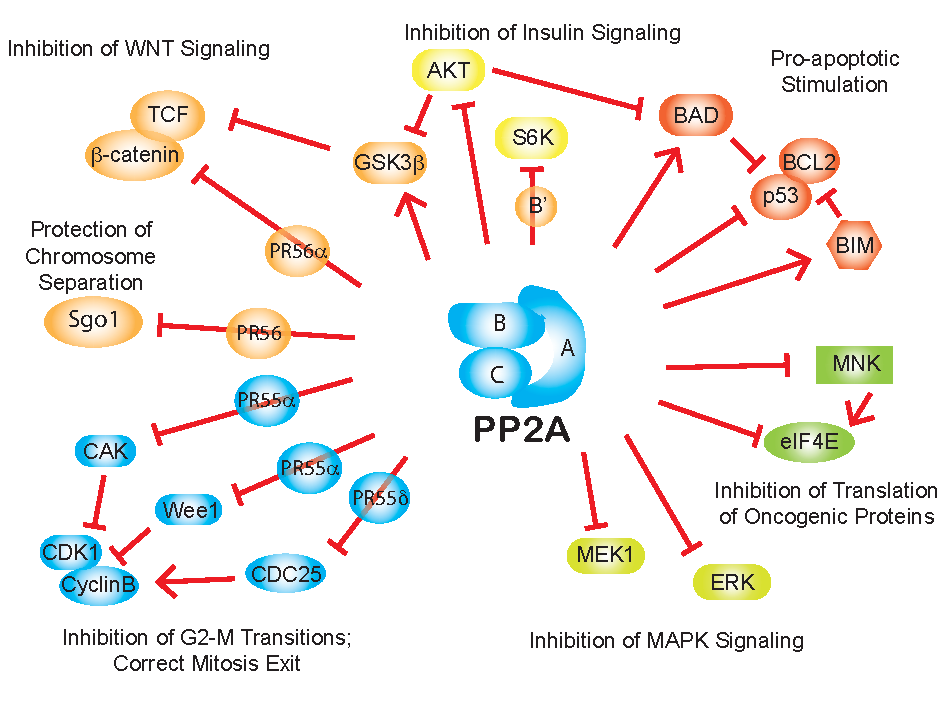
\includegraphics[width=1\textwidth]{figs/fig1-1 pp2a signaling.pdf}
\caption[PP2A in signaling]{\footnotesize PP2A is involved in many signaling pathways by counteracting phosphorylation events by many kinases. Adapted from Perrotti et al. \cite{perrotti_protein_2013}.}
\label{fig:fig1.1}
\end{figure}

\subsubsection{PP2A in metabolism}

Multiple PP2A regulatory subunits have been demonstrated to be involved in regulating the metabolism via the Insulin/\gls{akt}/\gls{mtor} signaling pathways. In \textit{Drosophila}, Hahn et al. demonstrated that PP2A regulatory B\textsuperscript{$\prime$} target S6K to modulate the phosphorylation of its activation site in our lab, and this regulation was conserved even in the Hela cell line \cite{hahn_pp2a_2010}. Another \textit{Drosophila} B\textsuperscript{$\prime$} subunit Widerborst modulates activated AKT via direct interaction and change the lipid droplet size and expression of lipid storage protein perilipin \cite{vereshchagina_protein_2008}. The C. \textit{elegans} B\textsuperscript{$\prime$} subunit pptr-1 could also directly regulate AKT's phosphorylation \textit{in vivo} and impact the life span, fat storage phenotype of worms \cite{padmanabhan_pp2a_2009}. 

In the mammalian system, AKT was also found to be associated with the PP2A--B55 holoenzyme, and its phosphorylation at Thr--308 was compromised by overexpressing PR55\textalpha{} subunit in both FL5.12 and NIH3T3 cells \cite{kuo_regulation_2008}. In 3T3-L1 adipocytes, over-expression of small t antigen, which generally inhibits PP2A activity, was found to have multiple impacts on the insulin pathway, including increased phosphorylation of insulin signaling downstream effector--AKT and GSK-3\textbeta{} \cite{ugi_protein_2004}. The inhibition of PP2A by the small t antigen in 3T3-L1 adipocytes enhanced the glucose uptake both in basal and insulin-stimulated condition. Another important master regulator in metabolism, the AMPK, was also found to be negatively regulated by PP2A \cite{wu_activation_2007,park_ampk_2013,wang_pp2a_2010}. In HepG2 cells, heat shock stress will dephosphorylate AMPK and enable to relieve the AMPK-mediated suppression on HSP70 expression \cite{wang_pp2a_2010}. And the AMPK inhibition after heat shock stress was shown to be mediated by PP2A. Intracellular calcium or palmitate could also inactivate AMPK via PP2A. The PP2A-B\textsuperscript{$\prime\prime$} subunit PR72 is known to have calcium binding sites, and could potentially be involved in intracellular calcium-mediated AMPK inhibition \cite{park_ampk_2013}. Excess fatty acid treatment, such as palmitate, could also inactivate AMPK via PP2A \cite{wu_activation_2007}.   

\subsubsection{PP2A in Wnt signaling}

In \textit{Xenopus}, B\textsuperscript{$\prime$} subunit PR56\textalpha{} was discovered to the negative regulator for the \textbeta-Catenin phosphorylation, which lead to the degradation of \textbeta-Catenin via the ubiquitin/proteasome pathway \cite{li_protein_2001}. However, recent evidences showed the PP2A has more complicated control in Wnt signaling \cite{eichhorn_protein_2009}. Before Wnt ligand binding, \textbeta-Catenin is located in destruction complex including \gls{apc}, AXIN, and GSK3\textbeta{}. The PP2A B subunits, PR61\textalpha{}-\textdelta{}, binds to either APC or AXIN to destabilizing the \textbeta-Catenin. However the mechanism is still not clear. Upon Wnt ligand binding, the Wnt downstream effector Naked, which causes a negative feedback on Wnt signaling, requires the PR72 for its negative regulation, and is repressed by the PR130 (alternative splicing form of the PR72). Additionally, both PR61\textepsilon{} and PR55 could enhance Wnt signaling by destabilizing the inhibitory GSK3\textbeta{} (Figure~\ref{fig:fig1.1}). 

\subsubsection{PP2A in MAPK signaling}

For MAPK kinase signaling cascades, PP2A has also both inhibitory and activating role \cite{eichhorn_protein_2009}. Depending on the different combination of PP2A complexes, almost all MAPK pathways can be negatively regulated \cite{junttila_phosphatase-mediated_2008}. Both \textit{in vivo} and \textit{in vitro} studies has shown that inhibition of PP2A increases ERK and MEK phosphorylation \cite{junttila_phosphatase-mediated_2008}. Furthermore, PR61\textbeta{} and PR61\textgamma{} directly de-phosphorylate ERK \cite{eichhorn_protein_2009} (Figure~\ref{fig:fig1.1}). PP2A was also shown to interact with Shc, the upstream regulator in MAPK signaling, and suppress its tyrosine phosphorylation and activation on MAPK signaling cascade \cite{junttila_phosphatase-mediated_2008}. 

Related to PP2A's activating role, PR55\textalpha{} binds and dephosphorylates KSR1 and RAF upon RAS activation. And this leads to the plasma membrane recruitment of RAF and subsequent enhanced binding between RAF and RAS, therefore stronger activation of MAPK signaling \cite{eichhorn_protein_2009}. On the other hand, PR55\textgamma{} interacts with c-SRC and inhibits c-SRC's positive regulation on RAF independently from RAS activation. 


\subsubsection{PP2A in apoptosis}

PP2A has also pro-apoptotic activity via its inhibitory effect on AKT, which inactivates the anti-apoptotic protein BCL2 and activates pro-apoptotic factors like BAD and BIM \cite{eichhorn_protein_2009,janssens_role_2012} (Figure~\ref{fig:fig1.1}). PP2A directly binds BCL2 and BIM and de-phosphorylates them. Also, PP2A directly binds to the BH4 domain of BCL2 and removes the phosphorylation at Ser70 of BCL2, which causes enhanced interaction between p53 and BCL2 to inhibit BCL2's anti-apoptotic function. Additionally, the inhibition of PP2A by okadaic acid or siRNA increases eIF4E phosphorylation via MNK kinase \cite{li_protein_2010}. These findings are consistent with the tumor suppressor role of PP2A.


\subsubsection{PP2A in cell cycle control}

PP2A has a fundamental role in controlling cell cycle. During G1--S transition, PR56\textgamma{} is translocated into the nucleus and PP2A terminal methylation levels also change \cite{eichhorn_protein_2009}. Also, PR55\textalpha{} is inhibiting CDK1-Cyclin B complex via the inhibition of \gls{cak} and Wee1 kinase. PR56\textdelta{} could also de-phosphorylate CDC25 and inactivate it. The PR56 family could also regulate sister chromatid cohesion, which is important for proper chromosome segregation in mitosis and meiosis \cite{hu_scaffold_2014,kitajima_shugoshin_2006}. In my own PhD thesis project, over-expression of mouse PP56\textgamma{} (PPP2R5C) in Hepa 1-6 has also resulted in dense chromosome in \gls{dapi} staining, which confirmed the B\textsuperscript{$\prime$} subunits' role in chromosome segregation (data not shown). 


\subsubsection{PP2A in cell proliferation}

PP2A has been demonstrated with multiple evidences for its tumor suppressor activity in the human cell transformation \cite{janssens_pp2a:_2005,mumby_pp2a:_2007}. Viral antigen SV40 small T antigen or tumor-inducing toxins like okadaic acid and microcystin-LR have been shown to be the viral or chemical inhibitor for PP2A activity \cite{campbell_identification_1995,nagao_protein_1995}. In addition, \textit{in vivo} inhibitor for PP2A CIP2A, an endogenous interacting protein for PP2A, has been found to be the stabilizer for c-Myc and mediating PP2A's inhibition in human malignancies \cite{khanna_cancerous_2013,junttila_cip2a_2007}. 

PP2A scaffold and regulatory subunits have been shown to be mutated or down-regulated in multiple cancers \cite{seshacharyulu_phosphatase:_2013}. Knockdown of PR56\textgamma{} in HEK cell inhibits PP2A phosphatase activity similar to the extent achieved by SV40 small T antigen and induces anchorage-independent tumor growth \cite{chen_identification_2004}. The PP2A PR56\textgamma{} containing holoenzyme has tumor growth suppression activity via de-phosphorylation on the p53 at Thr--55 \cite{li_specific_2007,shouse_serine_2008}, and leads to the growth arrest and inhibition of cell proliferation.

\section{Aim of study--PPP2R5C}

In our lab, homolog of PPP2R5C in Drosophila, \gls{PP2A}-B\textsuperscript{\ensuremath{\prime}}, has been previously shown that it regulates the organismal metabolism \cite{hahn_pp2a_2010} via directly de-phosphorylating \gls{s6k} in \textit{Drosophila}. In agreement with S6K activation phenotype, fly with \gls{PP2A}-B\textsuperscript{\ensuremath{\prime}} whole body knockout had increased insulin signaling phenotype, which was the decreased life span and whole body triglyceride. The initial study in Hela cell also shows that the human homolog of \gls{PP2A}-B\textsuperscript{\ensuremath{\prime}}, PPP2R5C, also negatively regulates the S6K phosphorylation. The naturally following question would be whether there is any link between PPP2R5C and metabolic status in more translational related context, such as in mice or human patients. 

The knockout mice in PPP2R5C results in heart development defects, including the formation of incomplete ventricular septum and a decrease in the number of ventricular cardiomyocytes \cite{varadkar_protein_2014}. In addition, PPP2R5C knockout mice have a decrease in locomotive coordination and gripping strength, which indicates that PPP2R5C is also required for efficient neuromuscular function. Finally, the knockout mice have also neonatal growth deficiency, but survived knockout mice develop obesity after weaning and have 31\% more body weight at the age of 6 months. However, the exact mechanism causing the obesity is still not clear. It could be a secondary consequence of reduced locomotive activity or active metabolic change in a certain metabolic relevant organ. The tissue-specific manipulation of PPP2R5C is needed for clarifying the multiple defects in whole-body knockout mice. 

Proteomic studies on PPP2R5C interacting partners reveals several interesting candidates as PPP2R5C's phosphatase substrates \cite{arroyo_liprin_2008,zhou_proteomic_2007}. A \gls{gst} tagged PPP2R5C was used to unravel its potential interaction partners by Mass Spectrometry approach \cite{zhou_proteomic_2007}. And several proteins, such as the calcium pump SERCA2a and SERCA3a, are involved in the calcium homeostasis. Interestingly, the SERCA2a has been recently identified as the Serpin-interacting protein and shown that SERCA2a homolog in \textit{Drosophilla} is required for the fat storage in fat body (primitive organ with function of the liver and adipose tissue in \textit{Drosophilla} \cite{hietakangas_regulation_2009}) \cite{bi_seipin_2014}, which could potentially be conserved in mice and fit with the obesity phenotype in PPP2R5C knockout mice \cite{varadkar_protein_2014}. The over-expression of PPP2R5C in cultured myocytes impairs the cell contractility \cite{zhou_proteomic_2007}. Another \gls{tap} tagged PPP2R5C based proteomic strategy also found the Liprin \textalpha{}1 is interacting with PPP2R5C independent of PP2A holoenzyme \cite{arroyo_liprin_2008}. Liprin \textalpha{}1 is suggested to stabilize PPP2R5C and regulate the focal adhesion \cite{arroyo_liprin_2008}. 

Human PPP2R5C has been shown to be involved in regulating p53 tumor suppressor activity upon DNA damage\cite{li_specific_2007,shouse_serine_2008}. After DNA damage, the PR56\textgamma{} containing PP2A holoenzyme binds p53 and de-phosphorylates Thr55 of p53, which leads to the induction of downstream transcriptional target p21 and following inhibition of cell proliferation \cite{li_specific_2007}. In addition, the interaction between PR56\textgamma{} and p53 upon DNA damage require the ATM-dependent phosphorylation of Ser15 in p53 \cite{shouse_serine_2008}. However, p53 protein sequence alignment between human and mouse shows that the Thr55 in mouse is missing, and this deletion rules out the possibility of mouse PR56\textgamma{}'s ability to inhibit the cell proliferation via p53. Indeed, PPP2R5C knockdown in mouse cell lines has very mild effects on proliferation (\textit{circa} 5\% increase in total protein content, data not shown).

Human PPP2R5C is also involved in \gls{tcr}-induced \gls{nfkb} activity \cite{breuer_protein_2014}. The \gls{nfkb} is activated upon T cell stimulation by complex phosphorylation event cascade. PPP2R5C was found to be the negative regulator to fine-tune and terminate the \gls{nfkb} activation. PPP2R5C silencing in stimulated primary human T cell causes increased phosphorylation in \gls{ikk} and \gls{ikba}. 

In this thesis project, I have explored the mammalian function of PPP2R5C in metabolism control by tissue-specifically manipulating the expression of PPP2R5C in metabolically relevant tissues, such as the mouse liver. In addition, I have also employed systematic approaches, such as the microarray analysis after PPP2R5C knockdown and the proteomic study of PPP2R5C's substrates, to investigate the potential mechanism behind PPP2R5C's metabolism control. 


